\label{chapter:sampling of the emission spectra}
The next step to set up the source is to calculate the decay probability of each decay path. For that, it is necessary to know the shape of the beta decay spectra for both samples. According to the atlas of the beta decay spectrum written by the \emph{Institute of Physics and Engineering in Medicine} \cite{BetaRayAtlas}, the spectrum is: 

\begin{figure}[!h]
\hspace{1.6cm}
\begin{subfigure}{0.4\textwidth}
    %\captionsetup{margin={20pt,0pt}}
    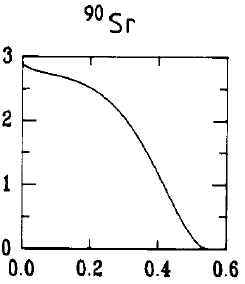
\includegraphics[scale = 0.6]{Master Thesis Manuel Galdon/figures/sr-90 decay spectrum.PNG} 
    %\caption{Decay spectrum of \ce{^{90}{}Sr}}
        %\label{fig:Sr-90_decay_spectrum}
\end{subfigure}
\hspace{1.6cm}
\begin{subfigure}{0.5\textwidth}
    %\captionsetup{margin={0pt,0pt}}
    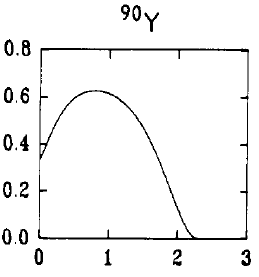
\includegraphics[scale = 0.6]{Master Thesis Manuel Galdon/figures/Y-90 decay spectrum.PNG}
    %\caption{Decay spectrum of \ce{^{90}{}Y}}
        %\label{fig:Y-90_decay_spectrum}
\end{subfigure}
    \caption{Number of beta particles emitted per \unit{\mega\electronvolt} for one transition of \ce{^{90}{}Sr} (left) and \ce{^{90}{}Y} (right).}
\label{fig:beta decay spectra of Sr and Y}
\end{figure}

Knowing the spectrum of both samples, it is therefore possible to sample the spectrum of emission for both of them and configure the source using multiple discrete energies together with their probability. To simplify the configuration of the source and avoid stepping into nested probability calculations, the simulation is executed twice: once for each sample whilst assuming 100$\%$ decay probability for \ce{^{90}{}Sr}, and once assuming 99.9885 $\%$ and 0.0115$\%$ decay probability for the processes $\ce{^{90}{}Y} \xrightarrow{\beta ^-} \ce{^{90}{}Zr}$ and $\ce{^{90}{}Y} \xrightarrow{\beta ^-} \ce{^{90}{}Zr^0+}$, respectively. Only the corresponding probabilities to the energy bins of the $\beta^-$ processes are taken into account at this point and they are taken from the \emph{International Atomic Energy Agency} \cite{intlAtomicEnergy}.

Once each simulation completes, the data for the particle flux and for the dependence of the deposited energy on the density of the corrosion layer is obtained. The data needs an additional \textbf{sampling} to account for the activity produced by each (strontium and yttrium) radiation source. As described before, roughly 50$\%$ of the total activity comes out of each sample. It is important to note that this last sampling is done after the simulation completes, which means that the only sampling included in MCNP is the sampling of energies that account for each decay path. This sampling make up the values of the next table:

\begin{table}[htbp]
  \begin{minipage}[t]{0.48\textwidth}
    \centering
    \begin{tabular}{|c|c|}
      \hline
      \rowcolor[HTML]{A9D9C6} 
      \multicolumn{1}{|l|}{\cellcolor[HTML]{A9D9C6}E [MeV]} & \multicolumn{1}{l|}{\cellcolor[HTML]{A9D9C6} $\beta^-$ Sr-90 [\%]} \\ \hline
      0.0137                                                   & 7.79                                                                      \\ \hline
      0.0410                                                    & 7.60                                                                      \\ \hline
      0.0683                                                    & 7.50                                                                      \\ \hline
      0.0956                                                    & 7.40                                                                      \\ \hline
      0.123                                                    & 7.30                                                                      \\ \hline
      0.150                                                    & 7.17                                                                      \\ \hline
      0.177                                                    & 7.01                                                                      \\ \hline
      0.205                                                    & 6.80                                                                      \\ \hline
      0.232                                                    & 6.53                                                                      \\ \hline
      0.259                                                    & 6.19                                                                      \\ \hline
      0.287                                                    & 5.78                                                                      \\ \hline
      0.314                                                    & 5.27                                                                      \\ \hline
      0.341                                                    & 4.68                                                                      \\ \hline
      0.369                                                    & 4.01                                                                      \\ \hline
      0.396                                                    & 3.27                                                                      \\ \hline
      0.423                                                    & 2.48                                                                      \\ \hline
      0.450                                                    & 1.71                                                                      \\ \hline
      0.478                                                    & 0.98                                                                      \\ \hline
      0.505                                                    & 0.43                                                                      \\ \hline
      0.532                                                    & 0.10                                                                      \\ \hline
    \end{tabular}
    \label{tab:decay probability of Sr-90}
  \end{minipage}%
  \hfill
  \begin{minipage}[t]{0.48\textwidth}
    %\vspace{\vfill} % Added to fix misalignment
    \centering
    \begin{tabular}{|c|c|}
      \hline
      \rowcolor[HTML]{A9D9C6} 
      \multicolumn{1}{|l|}{\cellcolor[HTML]{A9D9C6}E [MeV]} & \multicolumn{1}{l|}{\cellcolor[HTML]{A9D9C6} $\beta^-$ Y-90 [\%]} \\ \hline
      0.057                                                   & 4.26                                                                      \\ \hline
      0.171                                                    & 5.18                                                                      \\ \hline
      0.286                                                    & 5.94                                                                      \\ \hline
      0.400                                                    & 6.50                                                                      \\ \hline
      0.514                                                    & 6.87                                                                      \\ \hline
      0.628                                                    & 7.08                                                                      \\ \hline
      0.742                                                    & 7.17                                                                      \\ \hline
      0.857                                                    & 7.15                                                                      \\ \hline
      0.971                                                    & 7.04                                                                      \\ \hline
      1.080                                                    & 6.85                                                                      \\ \hline
      1.200                                                    & 6.57                                                                      \\ \hline
      1.310                                                    & 6.19                                                                      \\ \hline
      1.430                                                    & 5.69                                                                      \\ \hline
      1.540                                                    & 5.07                                                                      \\ \hline
      1.660                                                    & 4.30                                                                      \\ \hline
      1.770                                                    & 3.42                                                                      \\ \hline
      1.880                                                    & 2.46                                                                      \\ \hline
      2.000                                                    & 1.50                                                                      \\ \hline
      2.110                                                    & 0.64                                                                      \\ \hline
      2.230                                                    & 0.11                                                                      \\ \hline
    \end{tabular}
    \label{tab:decay_probability of Y-90}
  \end{minipage}
  \caption{Decay probabilities of strontium (left) and yttrium (right). In the Y-90 table, the decay to the ground excited state has not been included along with its probability.}
  \label{tab:sampling of Sr-90 and Y-90}
\end{table}


The values listed on Table \ref{tab:sampling of Sr-90 and Y-90} complete the definition of the source in MCNP after the probabilities are normalized to the unit. The decay path of the excited state is not included in the table although it is set in the definition of the source along with the values of Table \ref{tab:sampling of Sr-90 and Y-90}. Attending to the description of the decays of the \emph{International Atomic Energy Agency} \cite{intlAtomicEnergy}, the process $\ce{^{90}{}Y} \xrightarrow{\beta ^-} \ce{^{90}{}Zr^0+ } $ takes place at 184.6 \unit{\kilo\electronvolt} with a probability of 0.0115 $\%$. 

The next decay, $\ce{^{90}{}Zr^0+ } \xrightarrow{\gamma} \ce{^{90}{}Zr }$, is the only gamma decay that is considered in the analysis of the decay chain and happens at an energy of 1.76 \unit{\mega\electronvolt} \cite{intlAtomicEnergy}. Its probability, in turn, is taken as 100 $\%$ i.e. the same probability as for the process $\ce{^{90}{}Y} \xrightarrow{\beta ^-} \ce{^{90}{}Zr^0+ } $ i.e. 0.0115$\%$ since we are neglecting the most upper exited state pictured in Figure \ref{fig:Sr90_decay}. For this particular $\gamma$ transition, a separate line spectrum has been set up in MCNP to generate only photons. However, it is included in the bins of the input of MCNP to cover the excited state. The probabilities for $Sr-90$ and $Y-90$ that are listed on Table \ref{tab:sampling of Sr-90 and Y-90} are normalized to the unit and those are the values used in the MCNP source configuration.
